\documentclass[12pt]{article} % use larger type; default would be 10pt

%packages
\usepackage[utf8]{inputenc} % set input encoding (not needed with XeLaTeX)
\usepackage{fancyhdr}
\usepackage{float}
\usepackage{geometry}
\usepackage{ulem}
\usepackage{soul}
\usepackage{color}
\usepackage{graphicx}
\usepackage{hyperref}
\usepackage{array}
\usepackage{caption}
\usepackage{titling}
\usepackage{enumerate} 
\usepackage[dvipsnames]{xcolor}
\usepackage{amsmath}
\usepackage{amssymb}
\usepackage[compact]{titlesec}


 %put box around figure captions
\makeatletter
\long\def\@makecaption#1#2{%
  \vskip\abovecaptionskip
  \sbox\@tempboxa{\fbox{#1: #2}}%
  \ifdim \wd\@tempboxa >\hsize
    \fbox{\parbox{\dimexpr\linewidth-2\fboxsep-2\fboxrule}{#1: #2}}\par
  \else
    \global \@minipagefalse
    \hb@xt@\hsize{\hfil\box\@tempboxa\hfil}%
  \fi
  \vskip\belowcaptionskip}
\makeatother

%reduce space between 
\titlespacing{\section}{0pt}{*1}{*0}
\titlespacing{\subsection}{0pt}{*1}{*0}
\titlespacing{\subsubsection}{0pt}{*0}{*0}


%no indent and modify distance between paragraphs
\setlength\parindent{0pt}
\setlength\parskip{12pt}

%set margins and line spacing
\geometry{margin=1in}
\linespread{1.2}
\geometry{letterpaper}

%math operators
\DeclareMathOperator{\E}{\mathbb{E}}

%set up header and page numbering
\pagestyle{fancy}
\lhead{CS 155 Set 2}
\rhead{Timothy Liu}
\pagenumbering{arabic}



\title{CS155 Set 2}
\author{Timothy Liu}

\begin{document}

\maketitle

\newpage

\section{Problem 1}
\subsection{Problem A}
Square loss is a poor choice because a point that is correctly classified but has a predicted value far from the target will still register as a large loss. Square loss is very sensitive to extreme outliers.

\subsection{Problem B}

\begin{figure}[H]
	\makebox[\textwidth][c]{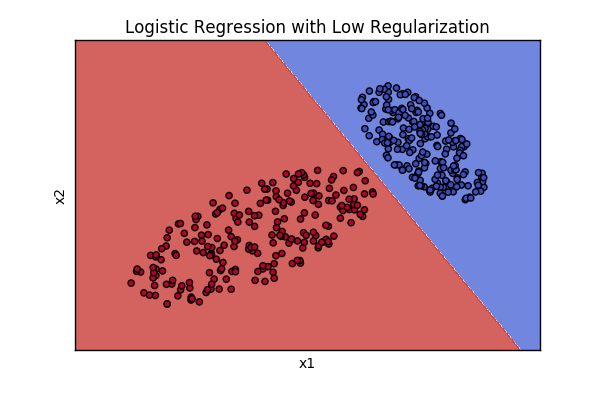
\includegraphics[width=4.2in]{log_reg.png}}
	\vspace{-10mm}
	\caption{Logistic regression with low regularization; C = 1000}
\end{figure}


\begin{figure}[H]
	\makebox[\textwidth][c]{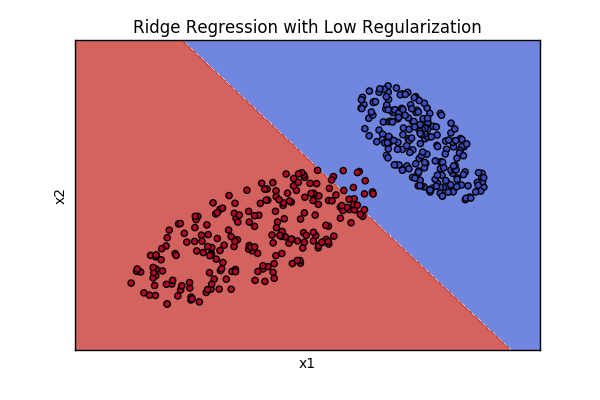
\includegraphics[width=4.2in]{ridge_reg.png}}
	\vspace{-10mm}
	\caption{Ridge regression with low regularization; alpha = 0.001}
\end{figure}

The ridge regression model misclassifies some points and is closer to the red points. The ridge regression classification line appears to be drawn closer to the center of mass of the red points, resulting in the misclassification.

\subsection{Problem C}
\underline{Gradient of hinge loss:}

$$\nabla L_{hinge} = \nabla max(0, 1 - y\textbf{w}^{T}\textbf{x})$$
if     $y\textbf{w}^{T}\textbf{x} > 1:$
$$\nabla L_{hinge} = 0$$
if     $y\textbf{w}^{T}\textbf{x}  < 1:$
$$\nabla L_{hinge} = \nabla 1 - y\textbf{w}^{T}\textbf{x}$$
$$ = - y \textbf{x}$$

\underline{Gradient of log loss:}
$$\nabla L_{log} = \nabla ln(1 + e^{-y\textbf{w}^T\textbf{x}})$$
$$= \nabla (1 + e^{-y\textbf{w}^T\textbf{x}}) \frac{1}{1 + e^{-y\textbf{w}^T\textbf{x}}}$$
$$=  \frac{-y e^{-y\textbf{w}^T}}{1 + e^{-y\textbf{w}^T\textbf{w}}}\textbf{x}$$






\begin{figure}[H]
	\makebox[\textwidth][c]{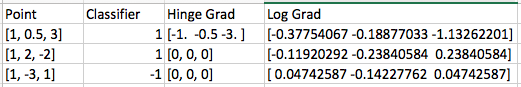
\includegraphics[width=4.2in]{1c.png}}
	\vspace{-10mm}
	\caption{Gradient of the weight vector for the hinge and log loss weight functions.}
\end{figure}

\subsection{Problem D}
The gradients from hinge loss are zero if the point is correctly classified or if the weight vector multiplied by x multiplied by the classification is at least 1. The log loss gradients are never zero, unlike the hinge loss functions. The log loss gradients will converge to zero when the product $yw^{\textbf{T}}x$ is very large (near infinity). The training error can be reduced by maximizing the margin.

\subsection{Problem E}
Minimizing only $L_{hinge}$ will result in a correct decision boundary; there may be multiple decision boundaries that have equivalent loss functions using hinge loss that have differing margins. Minimizing the term $\lambda||w||^2$ places a penalty on having a small margin and will result in a minimum margin, not just a correct decision boundary.

\section{Problem 2}
\subsection{Problem A}
Adding the penalty term will not decrease the in sample error. Without regularization, the model attempts to minimize the in sample error, but regularization is attempting to minimize a different quantity. 

Adding a penalty term will decrease the out of sample errors in cases where there is over-fitting in the training model. If the penalty term is excessively large and the out of sample set matches closely to the in sample set, then regularization will result in a higher out of sample error.

\subsection{Problem B}
The $L_0$ norm is rarely used because maximizing the $L_0$ norm is an NP-hard problem, making it computationally very challenging and inefficient. The $L_0$ norm is also not a continuous function.

\subsection{Problem C}

\begin{figure}[H]
	\makebox[\textwidth][c]{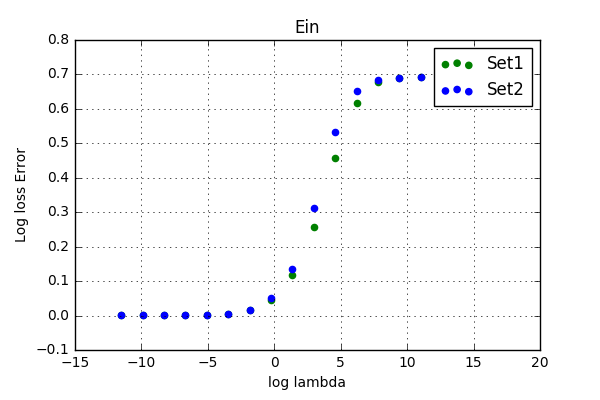
\includegraphics[width=4.2in]{Ein_reg.png}}
	\vspace{-10mm}
	\caption{In sample error for varying lambda.}
\end{figure}


\begin{figure}[H]
	\makebox[\textwidth][c]{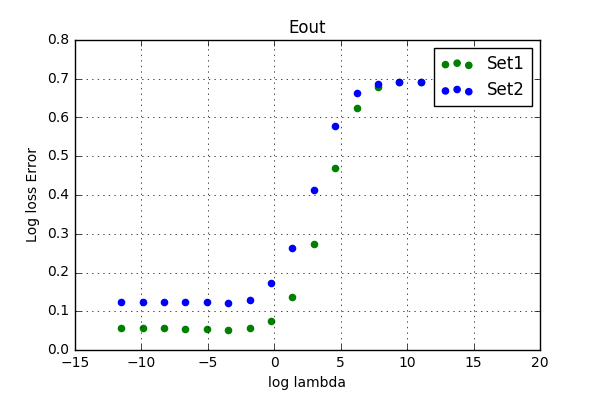
\includegraphics[width=4.2in]{Eout_reg.png}}
	\vspace{-10mm}
	\caption{Out of sample error for varying lambda.}
\end{figure}

\begin{figure}[H]
	\makebox[\textwidth][c]{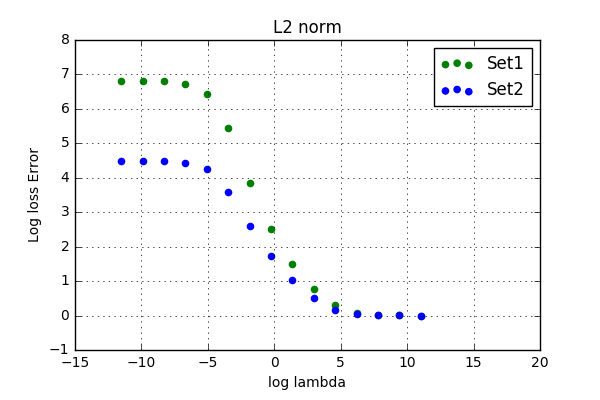
\includegraphics[width=4.2in]{norms_reg.png}}
	\vspace{-10mm}
	\caption{L2 norm for varying lambda.}
\end{figure}

\subsection{Problem D}
The training and errors for the two sets are almost identical. This is expected, since they are training off the same technique. The test errors for the larger dataset are consistently smaller. The larger training set is better able to generalize to the out of sample set, since the larger training set has a lower variance.

\subsection{Problem E}
The out of sample error for both test sets decreases slightly with larger lambda up to the sixth value of lambda for training set 1. Smaller values of lambda experience overfitting as the out of sample error rises even as the in sample error falls. Above this value of lambda, there is underfitting and the out of sample error rises significantly from the 8th to the 12th value of lambda.

\subsection{Problem F}
As $\lambda$ increases, L2 norm for training set 1 falls from about 48 to close to zero. As lambda increase, L2 norm first falls slowly before rapidly plummeting from the 4th to 9th lambda.

\subsection{Problem G}
For training set 2, $\lambda = 0.00125$ has the lowest test set error. This is the best choice of $\lambda$ if the data is trained on training set 2.

\section{Problem 3}

\subsection{Problem A}

\begin{figure}[H]
	\makebox[\textwidth][c]{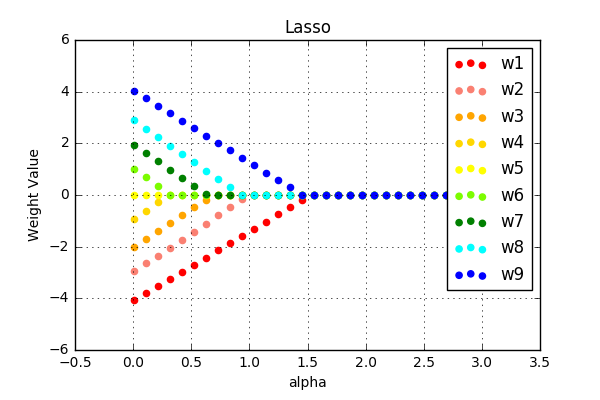
\includegraphics[width=4.2in]{lasso.png}}
	\vspace{-10mm}
	\caption{Value of weights as a function of alpha for lasso regularization.}
\end{figure}


\begin{figure}[H]
	\makebox[\textwidth][c]{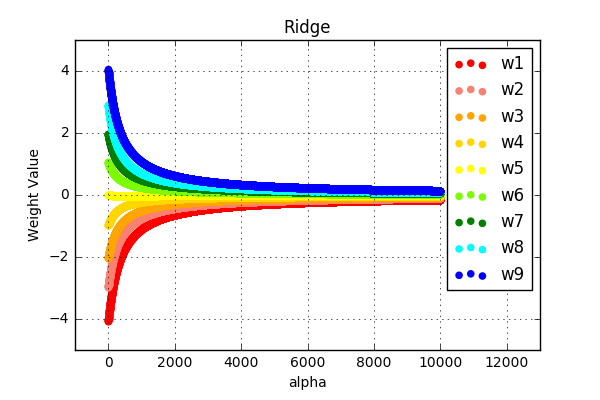
\includegraphics[width=4.2in]{ridge.png}}
	\vspace{-10mm}
	\caption{Value of weights as a function of alpha for ridge regularization.}
\end{figure}

As regularization increases, the number of model weights equal to zero increases for Lasso regularization. At $\alpha = 0$, exactly one model weight is zero. When $\alpha$ exceeds 1.5, all of the model weights are zero.

Ridge regression has none of the weights going to zero. The weights tend towards zero, but they don't converge to zero.

\subsection{Problem B}
\subsubsection{Problem i}

$$E_{in} = ||\textbf{y} - \textbf{x}w||^2 + \lambda||w||_1$$
$$\nabla E_{in} = -2\textbf{x}^T (\textbf{y} - \textbf{x}w) + \lambda  \frac{w}{||w||_1}= 0$$
$$\textbf{x}^T \textbf{y} - \textbf{x}^T\textbf{x}w - \frac{1}{2} \lambda  \frac{w}{||w||_1}= 0$$

For $w > 0$:
$$\textbf{x}^T \textbf{y} = \textbf{x}^T\textbf{x}w + \frac{1}{2} \lambda $$
$$\textbf{x}^T\textbf{x}w =  \textbf{x}^T \textbf{y} - \frac{1}{2} \lambda$$
$$w = (\textbf{x}^T\textbf{x})^{-1}(\textbf{x}^T \textbf{y} - \frac{1}{2} \lambda)$$

For $w<0$:
$$\textbf{x}^T \textbf{y} = \textbf{x}^T\textbf{x}w - \frac{1}{2} \lambda $$
$$\textbf{x}^T\textbf{x}w =  \textbf{x}^T \textbf{y} + \frac{1}{2} \lambda$$
$$w = (\textbf{x}^T\textbf{x})^{-1}(\textbf{x}^T \textbf{y} + \frac{1}{2} \lambda)$$
For $w=0$ we employ subgradients:
$$\nabla E_{in} = -2\textbf{x}^T (\textbf{y} - \textbf{x}w) +  [-1, 1] \lambda= 0$$
$$\textbf{x}^T \textbf{y} = \textbf{x}^T\textbf{x}w +  [-\frac{1}{2}, \frac{1}{2}] \lambda$$
$$\textbf{x}^T\textbf{x}w =  \textbf{x}^T \textbf{y} - [-\frac{1}{2}, \frac{1}{2}]  \lambda$$
$$\textbf{x}^T\textbf{x}w =  \textbf{x}^T \textbf{y} + [-\frac{1}{2}, \frac{1}{2}]  \lambda$$
$$w =  \textbf{x}^T\textbf{x}^{-1}(\textbf{x}^T \textbf{y} + [-\frac{1}{2}, \frac{1}{2}]  \lambda)$$




\subsubsection{Problem ii}

The weight vector is zero when 

$$(\textbf{x}^T \textbf{y} + [-\frac{1}{2}, \frac{1}{2}] \lambda) = 0$$

The smallest value that this occurs at is $\lambda = \pm2\textbf{x}^{T}\textbf{y}$. Since we are only considering positive $\lambda$, the $\pm$ is determined by whichever value will make $\lambda$ positive.

\subsubsection{Problem iii}
$$E_{in} = ||\textbf{y} - \textbf{X}\textbf{w}||^2 + \lambda||\textbf{w}||_2^2$$
$$E_{in} = ||\textbf{y} - \textbf{X}\textbf{w}||^2 + \lambda\textbf{w}^T\textbf{w}$$
$$\nabla E_{in} = ||\textbf{y} - \textbf{X}\textbf{w}||^2 + \lambda\textbf{w}^T\textbf{w} = 0$$
$$\textbf{X}^T(\textbf{y} - \textbf{X}\textbf{w}) + \lambda\textbf{w} = 0$$
$$\textbf{X}^T\textbf{y} - \textbf{X}^T\textbf{X}\textbf{w} + \lambda I\textbf{w} = 0$$
$$\textbf{X}^T\textbf{y} - (\textbf{X}^T\textbf{X} + \lambda I)\textbf{w} = 0$$
$$ (\textbf{X}^T\textbf{X} + \lambda I)\textbf{w} = \textbf{X}^T\textbf{y}$$
$$ \textbf{w} = (\textbf{X}^T\textbf{X} + \lambda I)^{-1}\textbf{X}^T\textbf{y}$$

\subsubsection{Problem iv}
No, there is no finite value for $\lambda$ that will give a weight value of zero. This is demonstrated in problem 3a.  In general, the matrix $\textbf{X}^T\textbf{X}$  is a symmetric matrix, and when the regularization term is added $(\textbf{X}^T\textbf{X} + \lambda I)$ is also a symmetric matrix. As $\lambda$ grows larger, there is no guarantee that the matrix $(\textbf{X}^T\textbf{X} +\lambda I)^{-1}$ will have any zero terms. If this matrix has no zero terms, then the product $ \textbf{w} = (\textbf{X}^T\textbf{X} + \lambda I)^{-1}\textbf{X}^T\textbf{y}$ is not guaranteed to lead to any zeros, meaning that there is no finite $\lambda$ that will necessarily lead to $w_i = 0$. $\lambda$ must be infinity for the weights to go to zero.














\end{document}
